\documentclass[../AnalysisNoteJBuxton.tex]{subfiles}

\renewcommand{\ResNum}{_3Res}
\renewcommand{\SaveNameModLamKch}{\MomRes\NonFlatBgd\ResNum\PrimMaxDecay\ResMethod\ParamFixAndShareLamKch}
\renewcommand{\SaveNameModLamKs}{\MomRes\NonFlatBgd\ResNum\PrimMaxDecay\ResMethod\ParamFixAndShareLamKs}

\begin{document}

\subsubsection{Results: \texorpdfstring{$\Lambda$K$^{0}_{S}$ and $\Lambda$K$^{\pm}$: 3 Residual Correlations Included in Fit}{TEXT}}
\label{ResultsLamK_3Res}

Figures \ref{fig:LamK0wConjFits_3Res}, \ref{fig:LamKchPwConjFits_3Res}, and \ref{fig:LamKchMwConjFits_3Res} (Section \ref{ResultsAndDiscussion}) show experimental data with fits for all studied centralities for \LamKs with \ALamKs, \LamKchP with \ALamKchM, and \LamKchM with \ALamKchP, respectively.
The parameter sets extracted from the fits can be found in Tables \ref{tab:FitResultsLamK0_3Res} and \ref{tab:FitResultsLamKch_3Res}.
All correlation functions were normalized in the range 0.32 $< k^{*} <$ 0.40 GeV/c, and fit in the range 0.0 $< k^{*} <$ 0.30 GeV/c.
For the $\Lambda$K$^{-}$ and $\bar{\Lambda}$K$^{+}$ analyses, the region 0.19 $< k^{*} <$ 0.23 GeV/c was excluded from the fit to exclude the bump caused by the $\Omega^{-}$ resonance.
The non-flat background was fit with a linear form from 0.6 $< k^{*} <$ 0.9 GeV/c.
The theoretical fit function was then multiplied by this background during the fitting process.

In the figures (\ref{fig:LamK0wConjFits_3Res}, \ref{fig:LamKchPwConjFits_3Res}, and \ref{fig:LamKchMwConjFits_3Res}), the black solid line represents the ``raw" fit, i.e. not corrected for momentum resolution effects nor non-flat background.
The green line shows the fit to the non-flat background.  The purple points show the fit after momentum resolution and non-flat background corrections have been applied.
The initial values of the parameters is listed, as well as the final fit values with uncertainties.

For the $\Lambda$K$^{0}_{S}$ fits without residuals, $\lambda$ was restricted to [0.4, 0.6].

\pagestyle{empty}
\begin{landscape}

\begin{figure}[h!]
  \centering
  %%----start of first subfigure---  
  \subfloat[Signal region view ($k^{*} \lesssim 0.3$ GeV/$c$)]{
    \label{fig:LamK0wConjFits_3Res:a}
    \includegraphics[width=0.50\linewidth]{\ResultsDirBaseLamKs\SaveNameModLamKs/canKStarCfwFitsLamK0wConj_0010_1030_3050\SaveNameModLamKs.pdf}}
  %%----start of second subfigure---
  \subfloat[Wide view ($k^{*} \lesssim 1.0$ GeV/$c$)]{
    \label{fig:LamK0wConjFits_3Res:b}
    \includegraphics[width=0.50\linewidth]{\ResultsDirBaseLamKs\SaveNameModLamKs/canKStarCfwFitsLamK0wConj_0010_1030_3050UnZoomed\SaveNameModLamKs.pdf}}  
  %%----overall caption----
  \caption[\LamALamKs Fits with 3 Residuals]{Fits, with 3 residual correlations included, to the \LamKs (left) and \ALamKs (right) data for the centralities 0-10\% (top), 10-30\% (middle), and 30-50\% (bottom).
The lines represent the statistical errors, while the boxes represent the systematic errors.
Each has unique $\lambda$ and normalization parameters.
The radii are shared amongst like centralities; the scattering parameters ($\mathbb{R}f_{0}$, $\mathbb{I}f_{0}$, $d_{0}$) are shared amongst all.
The black solid line represents the ``raw" fit, i.e. not corrected for momentum resolution effects nor non-flat background.  
The green line shows the fit to the non-flat background.
The purple points show the fit after momentum resolution and non-flat background corrections have been applied.
The initial values of the parameters is listed, as well as the final fit values with uncertainties.
Here, $R$ was restricted to [2.,10.] and $\lambda$ was restricted to [0.1,0.8].}
  \label{fig:LamK0wConjFits_3Res}
\end{figure}


\begin{figure}[h!]
  \centering
  %%----start of first subfigure---  
  \subfloat[Signal region view ($k^{*} \lesssim 0.3$ GeV/$c$)]{
    \label{fig:LamKchPwConjFits_3Res:a}
    \includegraphics[width=0.50\linewidth]{\ResultsDirBaseLamKch\SaveNameModLamKch/canKStarCfwFitsLamKchPwConj_0010_1030_3050\SaveNameModLamKch.pdf}}
  %%----start of second subfigure---
  \subfloat[Wide view ($k^{*} \lesssim 1.0$ GeV/$c$)]{
    \label{fig:LamKchPwConjFits_3Res:b}
    \includegraphics[width=0.50\linewidth]{\ResultsDirBaseLamKch\SaveNameModLamKch/canKStarCfwFitsLamKchPwConj_0010_1030_3050UnZoomed\SaveNameModLamKch.pdf}}  
  %%----overall caption----
  \caption[\LamKchPALamKchM Fits with 3 Residuals]{Fits, with 3 residual correlations included, to the \LamKchP (left) and \ALamKchM (right) data for the centralities 0-10\% (top), 10-30\% (middle), and 30-50\% (bottom).
The lines represent the statistical errors, while the boxes represent the systematic errors.  
Each has unique $\lambda$ and normalization parameters.
The radii are shared amongst like centralities; the scattering parameters ($\mathbb{R}f_{0}$, $\mathbb{I}f_{0}$, $d_{0}$) are shared amongst all.
The black solid line represents the ``raw" fit, i.e. not corrected for momentum resolution effects nor non-flat background.  
The green line shows the fit to the non-flat background.
The purple points show the fit after momentum resolution and non-flat background corrections have been applied.
The initial values of the parameters is listed, as well as the final fit values with uncertainties.}
  \label{fig:LamKchPwConjFits_3Res}
\end{figure}


\begin{figure}[h!]
  \centering
  %%----start of first subfigure---  
  \subfloat[Signal region view ($k^{*} \lesssim 0.3$ GeV/$c$)]{
    \label{fig:LamKchMwConjFits_3Res:a}
    \includegraphics[width=0.50\linewidth]{\ResultsDirBaseLamKch\SaveNameModLamKch/canKStarCfwFitsLamKchMwConj_0010_1030_3050\SaveNameModLamKch.pdf}}  
  %%----start of second subfigure---
  \subfloat[Wide view ($k^{*} \lesssim 1.0$ GeV/$c$)]{
    \label{fig:LamKchMwConjFits_3Res:b}
    \includegraphics[width=0.50\linewidth]{\ResultsDirBaseLamKch\SaveNameModLamKch/canKStarCfwFitsLamKchMwConj_0010_1030_3050UnZoomed\SaveNameModLamKch.pdf}}  
  %%----overall caption----
  \caption[\LamKchMALamKchP Fits with 3 Residuals]{Fits, with 3 residual correlations included, to the \LamKchM(left) with \ALamKchP (right) data for the centralities 0-10\% (top), 10-30\% (middle), and 30-50\% (bottom).
The lines represent the statistical errors, while the boxes represent the systematic errors.  
Each has unique $\lambda$ and normalization parameters.
The radii are shared amongst like centralities; the scattering parameters ($\mathbb{R}f_{0}$, $\mathbb{I}f_{0}$, $d_{0}$) are shared amongst all.
The black solid line represents the ``raw" fit, i.e. not corrected for momentum resolution effects nor non-flat background.  
The green line shows the fit to the non-flat background.
The purple points show the fit after momentum resolution and non-flat background corrections have been applied.
The initial values of the parameters is listed, as well as the final fit values with uncertainties.}
  \label{fig:LamKchMwConjFits_3Res}
\end{figure}


\begin{figure}[h]
  \centering
  \includegraphics[width=\textwidth]{\ResultsDirBaseLamKs\SaveNameModLamKs/Residuals\ResNum/LamK0/canKStarCfwFitsAndResidualsLamK0wConj_0010_1030_3050UnZoomed_ZoomResiduals\SaveNameModLamKs.pdf}
  \caption[\LamALamKs Fits showing 3 Residuals]{Fits, with 3 residual correlations included and shown, to the \LamKs (left) and \ALamKs (right) data for the centralities 0-10\% (top), 10-30\% (middle), and 30-50\% (bottom).  The three parent pairs used for the residual correction to the \LamKs (\ALamKs) fit are $\Sigma^{0}$K$^{0}_{S}$, $\Xi^{0}$K$^{0}_{S}$, and $\Xi^{-}$K$^{0}_{S}$ ($\bar{\Sigma}^{0}$K$^{0}_{S}$, $\bar{\Xi}^{0}$K$^{0}_{S}$, and $\bar{\Xi}^{+}$K$^{0}_{S}$).}
  \label{fig:LamK0wConjFitsAndResiduals_3Res}
\end{figure}




\begin{figure}[h!]
  \centering
  %%----start of first subfigure---  
  \subfloat[\LamKchPALamKchM fits with residual contributions shown for the centralities 0-10\% (top), 10-30\% (middle), and 30-50\% (bottom)]{
    \label{fig:LamKchwConjFitsAndResiduals_3Res:a}
    \includegraphics[width=0.50\linewidth]{\ResultsDirBaseLamKch\SaveNameModLamKch/Residuals\ResNum/LamKchP/canKStarCfwFitsAndResidualsLamKchPwConj_0010_1030_3050UnZoomed_ZoomResiduals\SaveNameModLamKch.pdf}}  
  %%----start of second subfigure---
  \subfloat[\LamKchMALamKchP fits with residual contributions shown for the centralities 0-10\% (top), 10-30\% (middle), and 30-50\% (bottom)]{
    \label{fig:LamKchwConjFitsAndResiduals_3Res:b}
    \includegraphics[width=0.50\linewidth]{\ResultsDirBaseLamKch\SaveNameModLamKch/Residuals\ResNum/LamKchM/canKStarCfwFitsAndResidualsLamKchMwConj_0010_1030_3050UnZoomed_ZoomResiduals\SaveNameModLamKch.pdf}}  
  %%----overall caption----
  \caption[\LamKchPALamKchM and \LamKchMALamKchP Fits with 3 Residuals]{Fits, with 3 residual correlations included and shown, to the \LamKchP \& \ALamKchM (left) and \LamKchM \& \ALamKchP (right) data for the centralities 0-10\% (top), 10-30\% (middle), and 30-50\% (bottom).  The three parent pairs used for the residual correction to the \LamKchP (\ALamKchM) fit are $\Sigma^{0}$K$^{+}$, $\Xi^{0}$K$^{+}$, and $\Xi^{-}$K$^{+}$ ($\bar{\Sigma}^{0}$K$^{-}$, $\bar{\Xi}^{0}$K$^{-}$, and $\bar{\Xi}^{+}$K$^{-}$).}
  \label{fig:LamKchwConjFitsAndResiduals_3Res}
\end{figure}




\end{landscape}
\pagestyle{plain}


%%%%%%%%%%%%%%%%%%%%%%%%%%%%%%%%%%%%%%%%     TABLES!!!!!     %%%%%%%%%%%%%%%%%%%%%%%%%%%%%%%%%%%%%%%%
\subfile{7_ResultsAndDiscussion/7.1.2_ResultsTables_3Res.tex}
%%%%%%%%%%%%%%%%%%%%%%%%%%%%%%%%%%%%%%%%%%%%%%%%%%%%%%%%%%%%%%%%%%%%%%%%%%%%%%%%%%%%%%%%%%%%%%%%%%%%%


\begin{figure}[h]
  \centering
  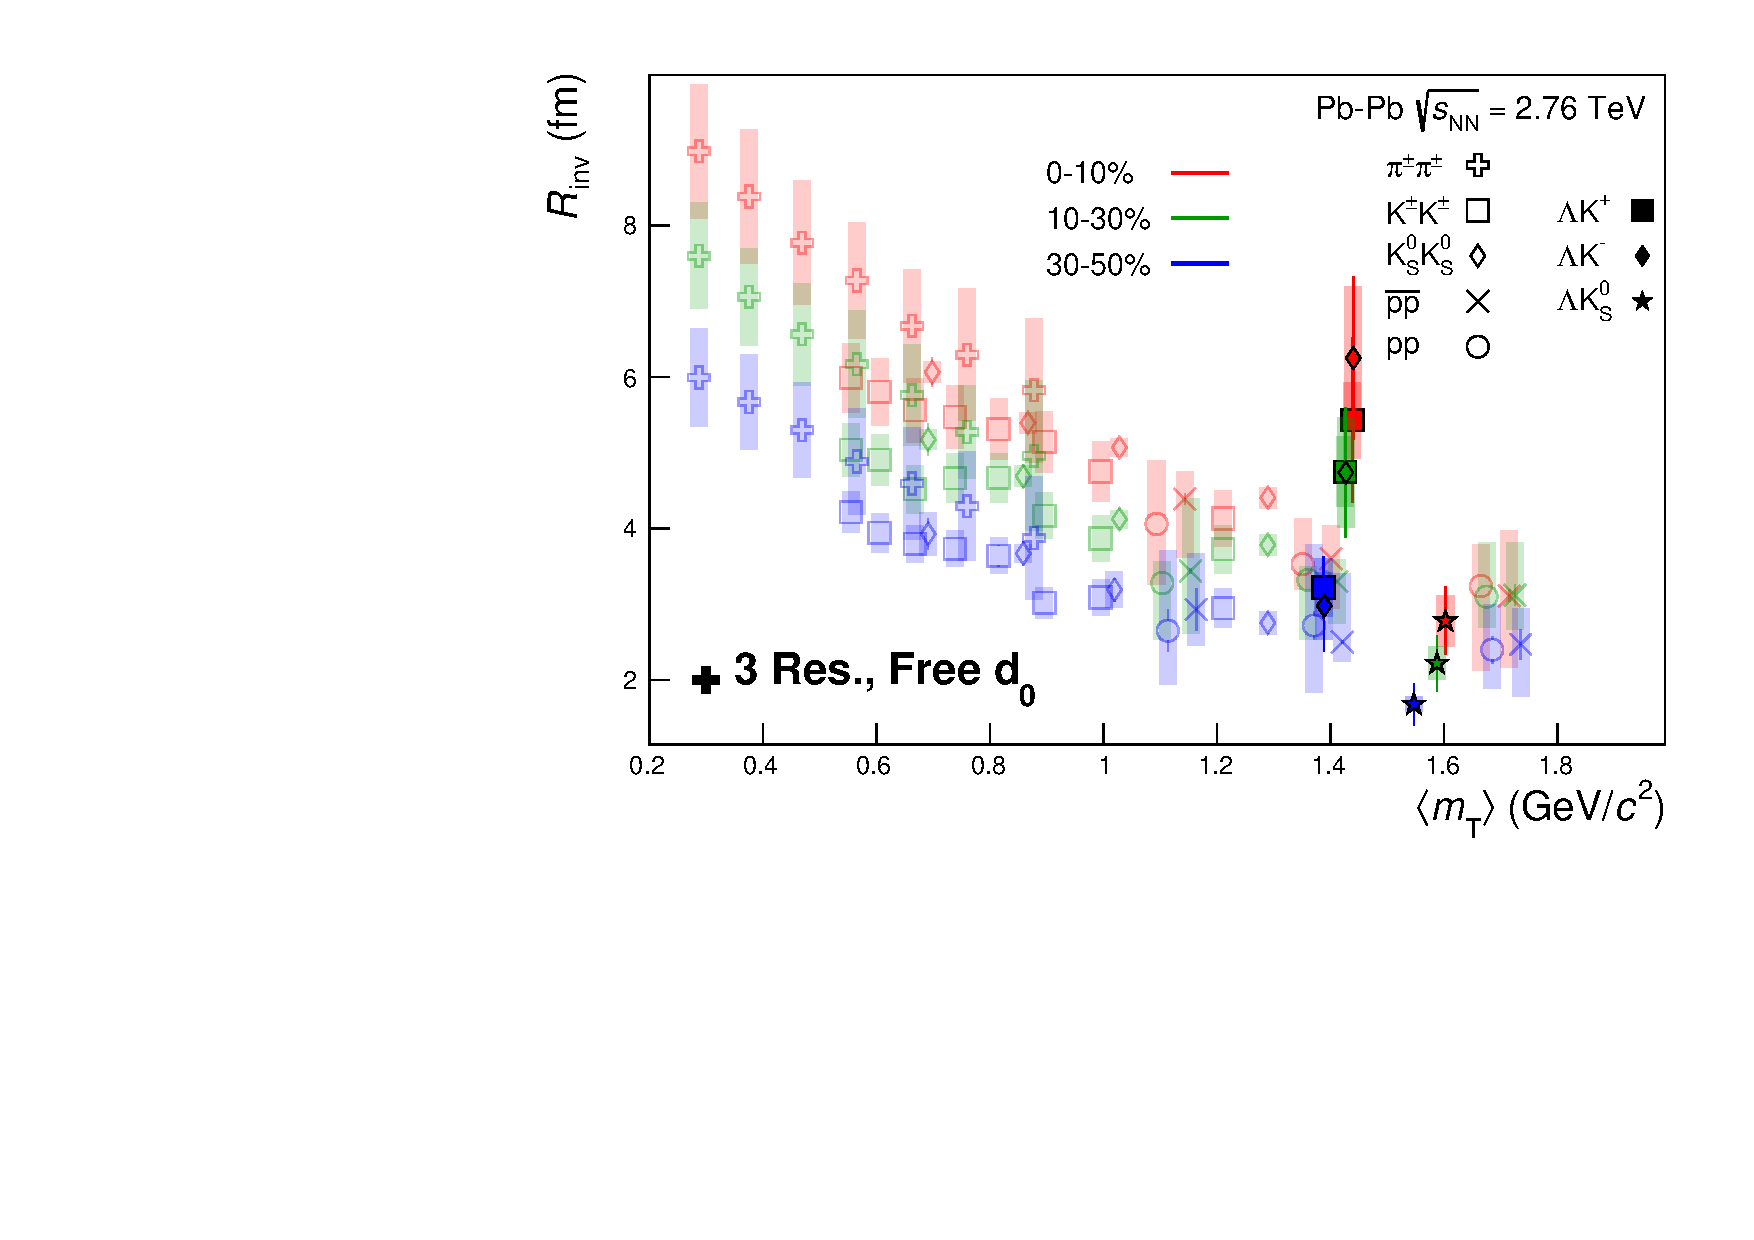
\includegraphics[width=\textwidth]{7_ResultsAndDiscussion/Figures/mTscaling_MinvCalc_OutlinedPoints_OthersTransparent_3Res_FreeD0.pdf}
  \caption[$m_{\mathrm{T}}$ Scaling of Radii: 3 Residuals in Fit]{3 residual correlations in \LamK fits.  Extracted fit $R_{\mathrm{inv}}$ parameters as a function of pair transverse mass ($m_{\mathrm{T}}$) for various pair systems over several centralities. The ALICE published data \cite{Adam:2015vja} is shown with transparent, open symbols.  The new $\Lambda$K results are shown with opaque, filled symbols.  In the left, the \LamKchP (with it's conjugate pair) results are shown separately from the \LamKchM (with it's conjugate pair) results.  In the right, all \LamKpm results are averaged.}
  \label{fig:mTScalingOfRadii_3Res}
\end{figure}

\clearpage





\end{document}